%%%%%%%%%%%%%%%%%%%%%%%%%%%%%%%%%%%%%%%%%%%%%%%%%%%%%%%%%%%%%%%%%%%%%%%%

%%% Empty Two Column LaTeX Template (Based on AAMAS-2023 (based on sample-sigconf.tex))

\documentclass[sigconf,nonacm]{acmart}

%%% Load required packages here (note that many are included already).

\usepackage{balance} % for balancing columns on the final page
\usepackage{float}
\usepackage{stfloats}
\usepackage[numbers]{natbib}

\newcommand{\argmax}{\mathop{\mathrm{argmax}}}

\title[RL Bachelor]{
    Assignment 1a: Exploration
}

\author{Peter Huijsen (s4516303) \& Ahmed Al Kurwi (s4476581)}
\affiliation{
    Group Number: 43
    \country{} \institution{} \city{} % Just included empty to avoid some warnings
}

%%%%%%%%%%%%%%%%%%%%%%%%%%%%%%%%%%%%%%%%%%%%%%%%%%%%%%%%%%%%%%%%%%%%%%%%

% Keep this part as is
\begin{document}
\pagestyle{fancy} 
\lhead{}
\rhead{Introduction to Reinforcement Learning, Leiden University, 2026}
\maketitle

%%%%%%%%%%%%%%%%%%%%%%%%%%%%%%%%%%%%%%%%%%%%%%%%%%%%%%%%%%%%%%%%%%%%%%%%

\section{Introduction}
In reinforcement learning (RL), an agent learns to make decisions by interacting with an environment, receiving feedback in the form of rewards or penalties over time.

This paper examines a simplified RL problem, namely the multi-armed bandit (MAB) problem.
In this problem, the environment consists of a single state with a set of actions, or arms, from which the agent can choose.
This only occurs once, and the agent receives a reward based on the action taken, without any further state transitions or interactions.

A crucial dilemma arises during this decision process, known as the exploration-exploitation trade-off dilemma. 
In this dilemma, agents must balance exploiting their current knowledge to maximize immediate rewards with exploring new actions to discover potentially better rewards in the future.

In this paper, three different MAB agents' approaches to this exploration-exploitation trade-off are compared: $\varepsilon$-greedy, Optimistic Initialization (OI), and Upper Confidence Bound (UCB).

\section{Methods}
First, the intuition and policies of each of these agents are described, before examining their performance.

\subsection{The Update Rule}
Each of these MAB agents learn from experience by updating its estimates after every interaction.
In most instances, the constant step size update rule is used:
% Q_n vs Q(a)
\begin{equation}
    Q(a)\leftarrow Q(a) + \alpha [R(a) - Q(a)]
\end{equation}
Here, $Q(a)$ is the estimated reward of the action $a$, $R(a)$ is the received reward of action $a$, and the term $[R(a) - Q(a)]$ is the prediction error. 
The prediction error is the difference between the expected and actual results for an action $a$. 
The $\alpha$ symbol is the constant step size and defines the learning rate of the agent; how much it should change its beliefs based on new information. As the name implies, this is a constant value. As such, more recently received rewards are weighed just as heavily as earlier received rewards.

Another version of the update rule is the sample average update rule, which decreases the weight of new information over time:
\begin{equation}
Q(a)\leftarrow Q(a) + \frac{1}{N(a)}[R(a) - Q(a)]
\end{equation}
Here, $N(a)$ is the number of times the action $a$ has been chosen thus far.
This means that earlier received rewards are weighed much more heavily than more recently achieved rewards. Therefore, this rule incentivizes near-term rewards.

\subsection{Naive and random agents}
The more advanced agents examined in this paper build upon the following two fundamental agents:
\begin{enumerate}
    \item \textbf{Naive/Greedy agent:} This agent always selects the action with the highest current $Q$-value. 
    It is efficient, but if it receives a small reward early by chance, it may never try other actions, possibly missing the optimal action.
    \item \textbf{Random agent:} This agent ignores its estimates and samples its actions from a uniform distribution with a probability of $\frac{1}{\mathcal{A}}$. 
    Here, $\mathcal{A}$ describes the set of actions the agent must choose from.
    Since it takes actions randomly, it cannot learn.
\end{enumerate}

\subsection{$\varepsilon$-greedy agent}
The way the $\varepsilon$-greedy policy balances exploration and exploitation is by occasionally choosing a random action. 
Still, the agent most often picks the optimal action based on its current beliefs.

Therefore, the $\varepsilon$-greedy agent selects an action based on the following policy:
\begin{equation}
    \pi_{\text{greedy}}(a) = 
    \begin{cases} 
    1 - \varepsilon, & \text{if } a=\argmax_{b\in\mathcal{A}}Q(b) \\
    \frac{\varepsilon}{|\mathcal{A}| - 1}, & \text{otherwise}
    \end{cases}
\end{equation}
Here, $\varepsilon\in[0,1]$ defines the exploration rate of the agent as a probability. 
For example, if $\varepsilon = 0.1$, the agent will spend $10\%$ of the time exploring and the other $90\%$ exploiting its current knowledge.

The agent uses the sample average update rule to rapidly converge to an estimation of the value of every action. This reduces the influence of later exploration.

\subsection{Optimistic Initialization agent}
This method uses high initial estimations to force the agent to explore. 
Instead of starting with $Q$-values at $0$, all estimations of action rewards are assigned to some optimistic value, e.g., $Q_{\text{initial}}=10$ in this scenario. 
When the agent then chooses an action $a$ and receives a more realistic reward, e.g., $R(a)=4$, the estimated reward for that action decreases. Thus, the greedy agent might choose a different action next with a higher estimated reward. This causes the agent to explore every action and rapidly converge to an optimal policy.

The agent uses the same greedy policy as the naive agent:
\begin{equation}
    \pi_{\text{OI}}(a)=\begin{cases}
        1, & \text{if } a=\argmax_{b\in\mathcal{A}}Q(b) \\
        0, & \text{otherwise}
    \end{cases}
\end{equation}

\subsection{Upper Confidence Bound agent}
The UCB agent explores based on uncertainty and confidence. 
If an action has not been tried many times, the uncertainty of the estimated reward is high. Then the agent considers the potential reward high. As such, the agent is more likely to choose this action next, since it chooses its actions based on this potential.

So, the agent selects the action $a$ by the following policy:
\begin{equation}
    \pi_{\text{UCB}}(a)=\begin{cases}
        1, & \text{if } a=\argmax_{b\in\mathcal{A}}\left[Q(b)+c\sqrt{\frac{\ln t}{N(b)}}\right] \\
        0, & \text{otherwise}
    \end{cases}
\end{equation}
Here, $t$ is the total number of steps taken and $c$ is the exploration constant. This constant controls how heavily the agent weighs the uncertainty of the estimated reward of an action. As an action is selected more often, $N_t(a)$ increases, this value decreases, and the agent relies more on the actual reward estimate ($Q$). However, as $t$ increases while the action is not selected again, the value increases.

This agent uses a constant step-size update rule; it has its own mechanism to account for time and uncertainty. 
In particular, if $N_t(a) = 0$, the uncertainty bonus becomes infinite, making sure that the agent tries every available action at least once before repeating any.

\begin{figure*}[t!]
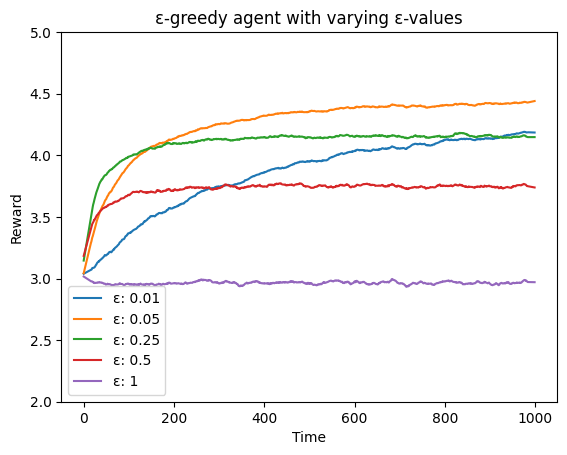
\includegraphics[width=0.32\linewidth]{figures/epsilon_greedy_lc.png}
\hfill
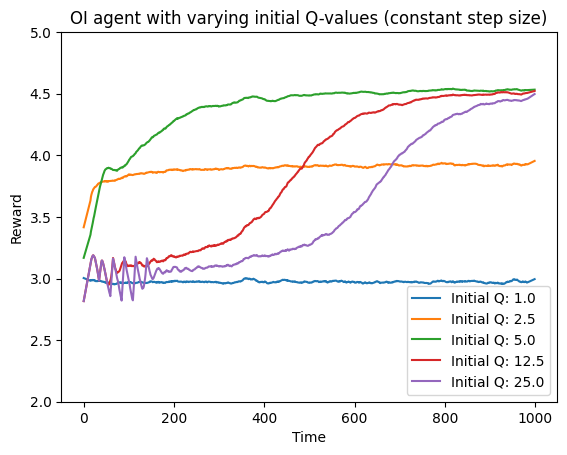
\includegraphics[width=0.32\linewidth]{figures/oi_lc.png}
\hfill
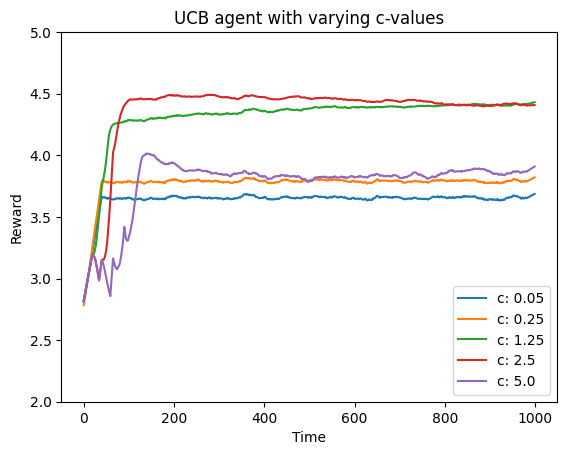
\includegraphics[width=0.32\linewidth]{figures/ucb_lc.png}
\caption{
    The learning curves of the $\varepsilon$-greedy, OI, and UCB agents. 
    The $\varepsilon$-greedy agents show a steady increase in performance over time for $\varepsilon<1$, with lower $\varepsilon$-values learning slower but achieving higher mean rewards in the long run. 
    For the OI agents, a higher $Q_{\text{initial}}$ value increases the time the agent explores and therefore increases the likelihood the agent finds the optimal policy before reverting to a naive policy.
    Finally, the UCB agents show stable increases in performance until $c=1.25$, thanks to their wider confidence levels. 
    This way the agent explores more before converging; however, with a too high $c$-value, exploration never stops. 
    The OI and UCB agents shown are using a constant step-size update rule with $\alpha=0.1$.
    The data shown was averaged over 500 runs, with 1000 timesteps.
}
\label{fig:performance}
\end{figure*}

\section{Results}
To accurately measure the performance of the different agents, each series of experiments was performed with varying hyperparameters to ensure representative performance. 

\subsection{Agent performance}
The learning curves of the $\varepsilon$-greedy, OI, and UCB agents with varying hyperparameters are shown in Figure~\ref{fig:performance}. For the $\varepsilon$-greedy agent, its performance is maximal for a relatively low $\varepsilon$-value of $\varepsilon=0.05$, but not a minimal $\varepsilon$-value. With this value, the agent learns the optimal policy more slowly than with a higher $\varepsilon$ value; however, when the agent finds the optimal policy, it will exploit it much more often than agents with a higher $\varepsilon$-value. This means that the mean reward for this agent will be higher than for those with a higher $\varepsilon$-value. It should be noted that the agent with $\varepsilon=0.01$ has not converged at $t=1000$, and as such may still achieve a higher mean reward.

The OI agent, in contrast, achieves a higher reward with a higher $Q_{\text{initial}}$-value. However, when this $Q_{\text{initial}}$ value is significantly large, it takes longer for the $Q$-values to converge to the optimal value. This is caused by the values of $Q_{\text{initial}}$ being significantly greater than the rewards that can be achieved. As such, a higher $Q_{\text{initial}}$ value encourages the agent to explore more actions before its policy converges to always choosing the near-optimal action. This is furthermore explained by the greedy action selection, which is identical to that of the naive agent, where the agent will always greedily determine its policy. 

However, in Figure~\ref{fig:oi}, the agents with a higher $Q_\text{initial}$ value do not take longer to converge. Since these agents are using the sample average update rule, the first range of updates to the $Q$ values is weighted more heavily, and as such, the values decrease more rapidly. The constant step-size update rule shown in Figure~\ref{fig:performance}, however, updates the $Q$-values more gradually, and as such explores more before exploiting the optimal action. 

\begin{figure}[H]
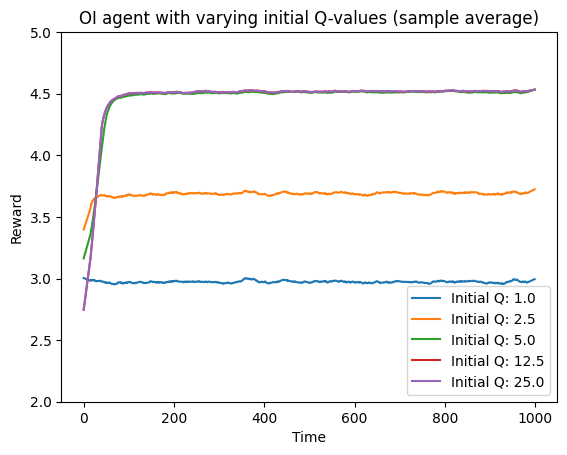
\includegraphics[width=0.64\linewidth]{figures/oi_lc_n.png}
\caption{The learning curve of the OI agents using a sample average update rule. The agents converge to their chosen policies faster than OI agents using the constant step-size update rule. Still, the values to which they converge remain similar. The red, green, and purple lines overlap.}
\label{fig:oi}
\end{figure}

Finally, the UCB agents in Figure~\ref{fig:performance} quickly converge to a set policy.
In these agents, the $c$-value determines the confidence level of the confidence interval from which it determines its policy. As such, agents with too low or too high $c$ values underperform when compared to an optimal policy. The confidence window is too restricted for low $c$-values, which causes the agent to not explore all arms enough to arrive at an optimal policy. It then behaves more like a naive agent, where it simply selects actions based on the highest mean $Q$-value. Similarly, too large a confidence window results in the agent not stopping with exploring since the confidence window does not tighten enough when selecting an action. The performance of the agent with $c=2.5$ also seems to decrease with time until it reaches the same performance as the agent with $c=1.25$. This can be explained by the uncertainty of earlier attempted actions resurfacing, and as such, makes the agent re-explore many actions to ensure its estimate of their reward. This decreases its performance over time, since it found the optimal policy early on, exploits it fully, and then decides to re-explore.

\subsection{Agent comparison}

\begin{figure*}[t!]
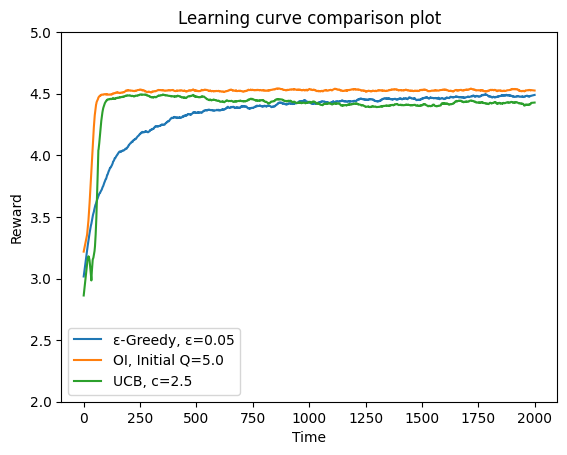
\includegraphics[width=0.32\linewidth]{figures/comparison_lc.png}
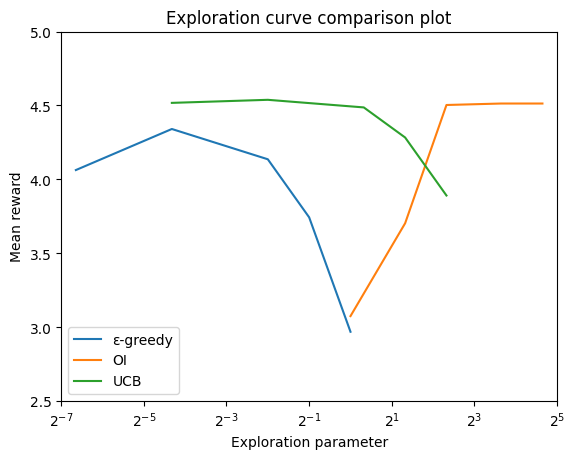
\includegraphics[width=0.32\linewidth]{figures/comparison_ec.png}
\caption{
    First, a comparison plot is shown of the learning curves for the $\varepsilon$-greedy, OI, and UCB agents. 
    The OI agent immediately reaches near-optimal performance, faster than the UCB agent, since its $Q$-values quickly converge, where afterwards it no longer explores and only exploits this optimal action. In contrast, the UCB and $\varepsilon$-greedy agents are still exploring in the end.
    Next, a comparison plot of the performance across exploration parameter values for each agent is shown. 
    In the exploration curve comparison plot, a clear peak of the mean reward of the agents is observed for their exploration parameter values.
    The exact parameter values used in the comparison plots for each agent are identical to those used for each agent of the same type in Figure~\ref{fig:performance}.
    The UCB agent shown uses a constant step-size update rule with $\alpha=0.1$, while the OI agent is using the sample average update rule. Each curve in every plot was averaged over 500 runs, with 2000 timesteps.
}
\label{fig:comparison}
\end{figure*}
The learning curves of each agent can be seen in a comparison plot in Figure~\ref{fig:comparison}.
The OI agent clearly performs best in this scenario, achieving its optimal performance the fastest and achieving a converged mean reward compared to the other agents. Both the UCB and OI agents converge rapidly, while the $\varepsilon$-greedy agent takes longer to reach this same level. Although the performance of the UCB agent decreases over time and is lower than that of the OI agent, it is more robust to changes in the environment. The optimistic values given to the OI agent are only given once; thus, if the rewards of the actions change, the agent is unable to handle this effectively. 

In the exploration curve comparison plot shown in Figure~\ref{fig:comparison}, there is a clear, optimal exploration parameter value for each agent. These exploration parameter values, through varying manners, define the proportion of actions that the agent chooses to explore or exploit. Therefore, since every agent is attempting to find the optimal action to exploit, while minimizing the actions it needs to explore, these values can neither be too low nor too high.  The agent either explores too little and converges to a policy in which it exploits a suboptimal action, or the agent continues to explore after it has found the optimal action.


\section{Discussion \& Conclusion}
This paper has shown a comparison of different MAB agents that approach the exploration-exploitation trade-off problem through different means. The UCB agent, using a confidence level to estimate expected action reward, rapidly learns to choose a near-optimal action and proceeds to primarily select this action. The OI agent achieves near-optimal action selection through greedily selecting its actions based on an optimistic initial $Q$-value after exploring and adjusting its $Q$-values for a considerable amount of time. The $\varepsilon$-greedy agent uses an $\varepsilon$-value to determine the proportion of actions in which the agent explores; however fails to exploit the optimal policy fully and therefore never reaches the same performance levels as the other agents.

The experiments conducted with these agents are limited in duration, and therefore, the performance of these agents could still improve after more time steps of simulation. Of note here is the $\varepsilon$-greedy agent, where the agent does not seem to have converged with $\varepsilon=0.01$. In addition, a limited range of discrete values for the exploration hyperparameters was chosen. As such, there could exist values for these hyperparameters that would result in different performance metrics than what was shown in this paper.

Future work could examine other agents that attempt to solve this exploration-exploitation trade-off in different ways than the models shown in this paper. An example of such an agent is a Thompson Sampling agent, which relies on Bayesian probability to model the reward distribution. Other future work could try to test these agents in a non-stationary environment. This could either drastically change the performance of each agent or not.

\newpage

\begin{figure*}[t!]
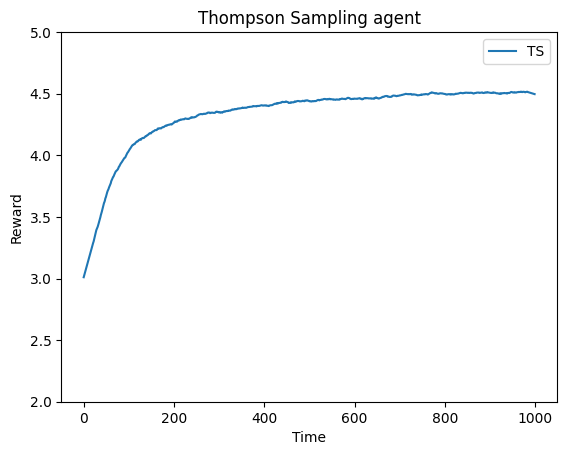
\includegraphics[width=0.32\linewidth]{figures/ts_lc.png}
\hfill
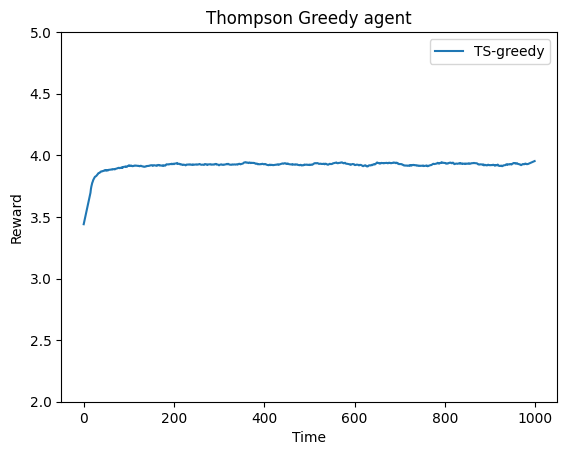
\includegraphics[width=0.32\linewidth]{figures/tsg_lc.png}
\hfill
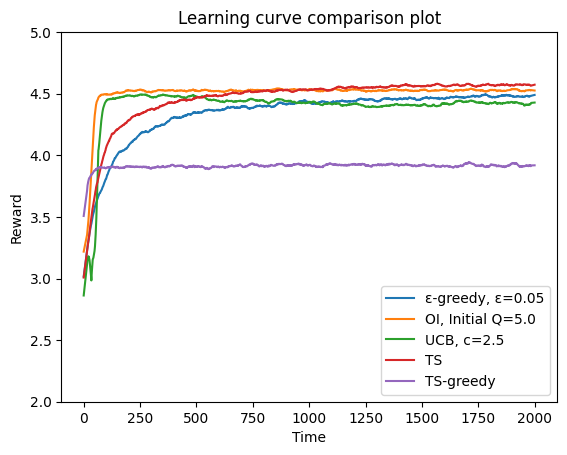
\includegraphics[width=0.32\linewidth]{figures/ts_comparison_lc.png}
\caption{
    The learning curve of the Thompson Sampling (TS) agent and the Thompson greedy agent. The figure also shows a comparison plot with the other agents shown in the rest of the paper. The TS agent performs better than the OI agent after 500 timesteps. Each curve was averaged over 500 runs, with 1 to 2000 timesteps. The reward distributions for each action in the environment for the Thompson agent quickly converge with minimal exploration, where afterwards the agent rapidly exploits the optimal action. The greedy Thompson agent does not sample from the action distributions and instead selects the action greedily based on the largest mean.
}
\label{fig:ts_performance}
\end{figure*}

\section{Extension}

This paper has covered a number of different algorithms that approach the exploration-exploitation trade-off differently. Another way to measure the confidence of an estimate is through Bayesian inference, where a probability distribution for each action keeps track of the respective confidence the agent has in the reward of each action. In this manner, when choosing an action and updating the reward distribution for the action, the agent gets more confident over time in the reward of the action. To calculate the probability of the action's optimality, Bayes' rule is used, where:
\begin{equation}
    P(A|B)=\frac{P(B|A)P(A)}{P(B)}
    \label{eq:bayes}
\end{equation}
In Equation~\ref{eq:bayes}, $P(A|B)$ is the posterior probability and defines the probability of a hypothesis $A$ given evidence $B$. This is calculated with the likelihood of the hypothesis $P(B|A)$, the probability of the prior knowledge $P(A)$, and the probability of the evidence $P(B)$.

In Thompson Sampling, the priors are modeled as a beta distribution, such that the prior of some action $a$ is defined as $\theta_a\sim \text{Beta}(\alpha_a,\beta_a)$ for $(\alpha_a,\beta_a) = (1,1)$. Given the total successes $\alpha_a$ and failures $\beta_a$, this beta distribution is then used to calculate the posterior of the hypothesis. Since this distribution is bounded between $[0,1]$, it is ideal to use in applications such as this, where the uncertainty needs to be modeled.

In the experiment shown in this paper, the reward received is $R(a)\in\{1,2,3,4,5\}$. To prevent the TS agent from converging too rapidly, these rewards need to be normalized such that we simply increment either $\alpha$ or $\beta$ for each action taken. Thus, $R'(a)=\dfrac{R(a)-1}{5-1}=\dfrac{R(a)-1}{4}$ is this normalized reward. To accommodate the Beta-Bernoulli framework laid out by \citet{russo2020tutorialthompsonsampling}, a single Bernoulli trial can be performed with success probability $R'(a)$. If this trial is a success, then $\alpha_a$ is incremented by 1; otherwise $\beta_a$ is incremented by 1. However, we could also simply update $\alpha$ and $\beta$ by the normalized reward, since the beta distribution is well defined for non-integer values:
\begin{equation}
    (\alpha_a,\beta_a)\leftarrow(\alpha_a+R'(a),\beta_a+(1-R'(a)))
\end{equation}

Then, when choosing an action, the TS agent can simply sample from the beta distribution for every action, and choose the action which has the maximum sample $\hat{\theta}_a\sim\text{Beta}(\alpha_a,\beta_a)$:
\begin{equation}
    \pi_\text{TS}(a)=\begin{cases}
        1, & \text{if } a=\argmax_{b\in\mathcal{A}}\hat{\theta}_b \\
        0, & \text{otherwise}
    \end{cases}
\end{equation}

The results from Figure~\ref{fig:ts_performance} show that while the OI agent converges much faster, the TS agent takes a slightly more gradual path and eventually reaches a near-optimal performance around a reward of 4.6 by roughly 500 steps, overtaking the OI agent. The Thompson greedy agent shows poorer performance compared to all the other agents, as its curve flattens out early at an average reward of about 4. This happens because it always picks the action with the highest expected value, making it get stuck on a good enough action. Like the Naive agent, it never explores enough to find the actual best action.

This figure also compares the TS agent and the TS-greedy agent with OI, UCB, and $\varepsilon$-greedy agents. Thompson Sampling is a strong way to handle the exploration-exploitation trade-off problem, because it relies on randomness shaped by experience. It explores efficiently without easily being tricked by, for example, initial high values, unlike Thompson greedy, which relies solely on the expected value (mean) of its Bayesian beliefs and does not use uncertainty, causing it to get stuck when it receives a good enough value.

The TS agent's $\alpha$ and $\beta$ counters grow forever, making its beliefs extremely rigid as time goes on. If the true rewards of the environment were to change, the agent would be too confident in its old knowledge to adapt quickly. This makes the TS agent struggle in non-stationary environments. Future work could try to add a forgetting mechanism, like a discount factor for the counters, so the agent forgets old data and stays flexible enough to find new optimal actions when the environment changes.

\bibliographystyle{plainnat}
\bibliography{bibliography}

%%% The following command should be issued somewhere in the first column 
%%% of the final page of your paper.
\balance

%%%%%%%%%%%%%%%%%%%%%%%%%%%%%%%%%%%%%%%%%%%%%%%%%%%%%%%%%%%%%%%%%%%%%%%%

%%% The next two lines define, first, the bibliography style to be 
%%% applied, and, second, the bibliography file to be used.

\end{document}

%%%%%%%%%%%%%%%%%%%%%%%%%%%%%%%%%%%%%%%%%%%%%%%%%%%%%%%%%%%%%%%%%%%%%%%%
